 
\graphicspath{{chapters/paper2/figures/}}


\chapter{Paper 2: \\Estimating cardiac contraction through high resolution data
  assimilation of a personalized mechanical model}

% \clearpage
\newpage
\section*{Estimating cardiac contraction through high resolution data
  assimilation of a personalized mechanical model}

\begin{center}
  Henrik Finsberg
  Gabriel Balaban,
  Stian Ross,
  Trine H\r{a}land,
  Hans Henrik Odland, 
  Joakim Sundnes, and
  Samuel Wall
\end{center}

 
\subsection*{Abstract}
% \begin{abstract}
  
Cardiac computational models, individually personalized, can provide
clinicians with useful diagnostic information and aid in
treatment planning.  A major bottleneck in this process can be  
determining model parameters to fit created models to individual
patient data. However, adjoint-based data assimilation techniques can
now rapidly estimate high dimensional parameter sets.  This method is
used on a cohort of heart failure patients, capturing cardiac mechanical
information and comparing it with a healthy control group.  Excellent
fit ($R^2 \geq 0.95$) to systolic strains is obtained, and analysis
shows a significant difference in estimated contractility between the
two groups.


% \clearpage
\newpage
%% main text
\section{Introduction}
\label{sec:introduction}

Patient-specific cardiac modeling has emerged as a potential tool
for clinical diagnosis as well as treatment
 optimization\cite{viceconti2016virtual}.  By linking
patient measurements to physical processes through a mathematical
framework, models can provide us with additional insight into
cardiac function or dysfunction at the level of the
individual. However, the complexity of the heart makes this difficult,
and this is recognized as a key challenge in modern bioengineering
\cite{hunter2010vision}. 

One difficulty is the effort to personalize models and
simulations to individual patients.  While a wealth of clinical 
data exists to parameterize such 'patient-specific' models, methods to
assimilate this data into simulations can involve extensive
computation time, often putting them outside the scope of clinical
utility. However, new methods are emerging to improve the flow of clinical
measurements into powerful data driven simulations.  Automated
geometry segmentation \cite{rabben2010technical} and improved
optimization techniques \cite{chabiniok2012estimation}, can improve the
speed at which patient-specific models can be built and parameterized.
In particular, recent advancements in adjoint-based data assimilation
techniques \cite{balaban} offer an efficient way to assimilate ventricular mechanical
 information using highly spatially resolved parameters.  
 
Here we use an adjoint based assimilation method with a mechanical
model in order to construct simulations that 
accurately reflect clinical motion data, both for
healthy controls and patients suffering from left bundle
branch block (LBBB). The use of a highly spatially resolved
contraction parameter, enabled through adjoint-methods, provides
excellent data fit to measured strains and volumes, and fit models
provide estimates of cardiac contraction. Such biomarkers may prove
useful to clinicians for diagnoses of problems with cardiac function,
and to better plan therapies.    

\section{Materials and methods}
\label{sec:methods}

\subsection{Data acquisition}
\label{sec:clinical_data}

Clinical measurements of cardiac function for seven LBBB patients were
obtained from the Impact study \cite{ImpactStudy2016}.
Data was also acquired for seven healthy volunteers. 4D echocardiographic
images of the left ventricle (LV), for both the LBBB patients and
healthy subjects, were captured using
a GE Vingmed E9 device, and analysis carried out with the
software package EchoPac. For each subject, depending on frame rate and cardiac cycle time, the
analysis provided between 15 and 50 LV volumes,  geometric segmentations of the LV
endocardium and epicardium, and cardiac strain calculated via speckle
tracking. The strain were defined according to
the 17 segment AHA-zone representation
\cite{cerqueira2002standardized}, in the longitudinal, radial and
circumferential direction, giving a total of 51 strain measurements
per time point, with the reference time point for strain analysis
  being the first frame after onset of QRS.

The LBBB patients had LV pressure measurements taken during
implantation of a cardiac resynchronization therapy (CRT) device, and
valvular events were used to synchronize the pressure to the echo
data. In the healthy control group, where invasive pressure measurements were
absent, the pressure waveform from one of the LBBB patients was used and
scaled to reported values of the end-diastolic and end-systolic
left ventricular pressure [Table 30-1 in \cite{klingensmith2008washington}].


\subsection{Automated geometry and microstructure creation}
For each patient, a 3D tetrahedral mesh of the LV was
constructed from triangulated segmented surfaces of the endo- and
epicardium corresponding to the frame at the beginning of
atrial systole, Figure \ref{fig:pipeline}. A cut was made at the
ventricular base of the segmentation, so that the mesh cavity volume
and the ultrasound measured volume differed by less than  $1$ ml. Mesh
cells were marked into the 17 AHA regions through the regionally
delineated strain data, and the myocardial fiber orientation, denoted
by $\ef$, were assigned using the algorithm from Bayer et al \cite{bayer2012novel},
with the endo- and epicardial helix fiber angles set to
$\alpha_{\text{endo}} = 60$ and $\alpha_{\text{epi}} = -60$, respectively.

\subsection{Mechanical Model}
We represent the heart as a hyperelastic continuum body, where the coordinates in
the reference ($\Xvec$) and the current ($\xvec$) configuration are
related via the displacement field $\uvec = \xvec-\Xvec$. Furthermore,
we utilize the
deformation gradient, the determinant of the deformation gradient
and, the right Cauchy-Green deformation tensor given by $\F= \I+\nabla
\uvec $,  $J = \det \F$ and $\C = \F^T\F$, respectively. 
% Constitutive relations
To model the passive behavior of the myocardium, the transversely 
isotropic strain energy function proposed in  \cite{holzapfel2009constitutive} is adopted:
\begin{align}
\label{eq:hoa}
  \mathcal{W}(I_1, I_{4\ef}) = \frac{a}{2 b} \left( \exp\left\{ b (I_1 
  - 3)\right\}  -1 \right)
  + \frac{a_f}{2 b_f} \left( \exp\left\{ b_f (I_{4\ef} 
  - 1)_+^2\right\} -1 \right).
\end{align}
Here $I_1 = \tr \C$ and $I_{4\ef}= \ef \cdot (\C \ef)$ are invariants
of $\C$, $(\cdotp)_{+}  = \max\{\cdot, 0\}$, and $a, a_f, b, b_f$ are
material stiffness parameters defining the elastic properties of the myocardium.
% Incompressibility
We follow a common approach and assume that the myocardium is incompressible. 
Incompressibility is incorporated in the model by using a two-field variational 
approach, where we introduce a Lagrange multiplier $p$ which represents the 
hydrostatic pressure, and the term $p(J-1)$ is added to the strain-energy.

% Active response
To model the active response we apply the approach of active strain
\cite{ambrosi2012active}, which is based on decomposing
the deformation gradient into active and passive contributions, $\F =
\F_e \F_a$. We choose $\F_a = (1 - \gamma) \ef \otimes \ef +
\frac{1}{\sqrt{1 - \gamma}} (\I - \ef \otimes \ef)$, where $\gamma$
is a parameter that represents the relative active shortening along
the fibers. For reference, we have also performed tests with the
commonly used active stress formulation, where the stress tensor 
is additively decomposed into active and passive stress $\sigma =
\sigma_p + \sigma_a$. Here $\sigma_p$ is
the elastic material response, and $\sigma_a = T_a \Fef \otimes \Fef$ with
$\Fef = \F\ef$ and $T_a$ a scalar variable representing active fiber
tension.


For both approaches, the resulting displacement field $\uvec$ and hydrostatic pressure $p$
are determined by using the principle of stationary potential energy
\cite{holzapfel2000nonlinear}, which is based on minimizing the total
energy  $\Pi(\uvec, p)$, which includes internal energy derived from
\eqref{eq:hoa} and external energy. The external energy includes
contributions from the measured cavity pressure $p_{\text{LV}}$, and a
linear spring term at the basal boundary, with spring constant
$k$ = 10.0 kPa. The equilibrium solution is found by solving for the minimum
potential energy, $\delta\Pi(\uvec, p) = 0$. 

\subsection{Data Assimilation}
In order to constrain the model to each patient's clinical measurements, we
consider a PDE-constrained optimization problem where
the objective functional is given by the misfit between
simulated and measured strain and volume along with a first order Tikhonov regularization of the
model parameters.
\begin{equation}
  \begin{aligned}
    \label{eq:pde_opt}
    & \underset{m}{\text{minimize}}
    & &  \alpha \left( \frac{V^i - \tilde{V}^i}{V^i} \right)^2
    + (1-\alpha)  \sum_{j= 1}^{17} \sum_{k \in \{c,r,l\}}  \left( \varepsilon_{kj}^i
      -  \tilde{\varepsilon}_{kj}^i \right)^2
    + \lambda \| \nabla m^i \|^2 \\
    & \text{subject to}
    & & \delta \Pi(\uvec, p) = 0.
  \end{aligned}
\end{equation}


Here $V$ and $\varepsilon_{kj}$ are the measured volume and regional Lagrangian strain in
segment $j$ in direction $k$ respectively, and $\tilde{V}^i =
-\frac{1}{3} \int_{\partial \Omega_{\text{endo}}} (\Xvec + \uvec)
\cdotp J\F^{-T}\Nvec  \mathrm{d}S$,  and $\varepsilon_{kj} =
\frac{1}{|\Omega_j|}\int_{\Omega_j}  \mathbf{e}_k^T \nabla \uvec \,
\mathbf{e}_k  \mathrm{d}x.$ 
The parameters $\alpha$ and $\lambda$
control the weights on the different terms, and the sum in the second
term is taken over the seventeen AHA
segments, and the three different strain components (Section \ref{sec:clinical_data}).


The data assimilation procedure is divided into two phases; a passive
and an active phase. For the passive phase we iteratively
  estimate the unloaded configuration and the linear isotropic parameter, $a$ in
\eqref{eq:hoa}, using an algorithm similar to the one described in
\cite{nikou2016effects}, and we set $\alpha= 1.0$,  with $\lambda = 0$ and
$\gamma = 0$, minimizing only the misfit with the measured volumes. The
remaining material parameters are fixed according to [Table 1 row 3 of
\cite{holzapfel2009constitutive}]. For the active phase we fix the material parameter optimized in the
passive phase, choose the control variable $m$ to be $\gamma$ or
$T_a$ for the active strain and active stress model respectively, and
set $\alpha = 0.95$ and $\lambda = 0.01$. This choice of $\alpha$ and
$\lambda$ was based on the analysis done in \cite{balaban}. A summary
of our optimization pipeline is provided to the right in
Figure~\ref{fig:pipeline}.





\begin{figure}[htbp]
\centering
    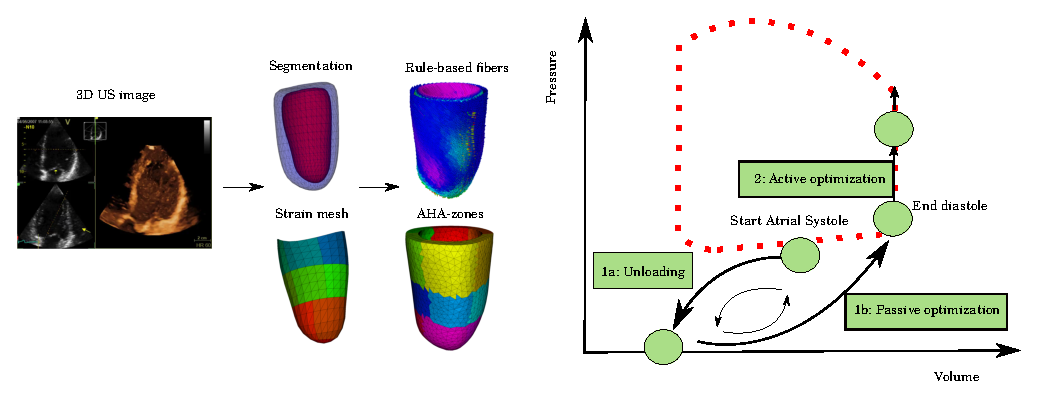
\includegraphics[width=\textwidth]{models}
\caption{Left: Automated anatomical modeling pipeline to produce AHA
  marked simulation meshes with applied fiber orientations from 3D
  echocardiographic segmentations. Right: Optimization
  pipeline. 1. Unloaded geometry and the linear isotropic
  material parameter $a$ in \eqref{eq:hoa} are estimated iteratively. The unloaded geometry is
  estimated based on the backward displacement method (1a)
  \cite{nikou2016effects} and $a$ is estimated by minimizing the
  difference between simulated and measured volumes (1b). 2. The unloaded
  geometry and the material properties are fixed, and the amount of
  contraction ($\gamma$ for active strain and $T_a$ for active stress)
  is estimated by minimizing the mismatch between simulated and
  measured strain and volume. The active optimization continues to the
  next measurement point until all measurement points in the cycle are covered.}
\label{fig:pipeline}
\end{figure}

\subsection{Implementation details}
We employ a Galerkin finite element method with Taylor-Hood
tetrahedral elements, that is $(\uvec, p) \in \mathbb{P}_2 \times
\mathbb{P}_1 $, with $\mathbb{P}_n$ being the space of piecewise
polynomials of degree $n$.
The solver is implemented in the finite element framework FEniCS
\cite{logg2012automated}, and uses a Newton trust region algorithm
\cite{PETScPackage} to solve nonlinear systems. The minimization of the
model-data misfit functional~\eqref{eq:pde_opt} is accomplished by a sequential
quadratic programming algorithm (SQP)~\cite{kraft1988software}, where
the functional gradient is computed by solving an automatically derived adjoint
equation \cite{farrell2013automated}. In these minimizations an upper
bound of $0.5$ and $500$ kPa is set for the active strain ($\gamma$)
and active stress ($T_a$) control variable respectively, which both
are modeled as functions in $\mathbb{P}_1$, yielding one parameter per
nodal point in the mesh.

\subsection{Contraction analysis}
Although direct physical interpretation of the active
  strain parameter $\gamma$ is difficult, it may be seen as the
  relative shortening of an isolated and unloaded muscle cell. A high
  value of $\gamma$ is therefore an indication of higher contractile
  force in the myocardium, independent of load. We propose that
  the spatially averaged $\gamma$ over the entire LV, denoted by  
  $\overline{\gamma}$, can be used as an index of global
  contractility. Similarly, the active stress parameter $T_a$ is related to force
  development at level of the sarcomeres\cite{goktepe2014generalized},
  and the spatially averaged 
  $T_a$, denoted $\overline{T_a}$ can be used as an index of
  contractility. In addition to the contractility information contained in 
$\overline{\gamma}$ and $\overline{T_a}$, the overall elastic state
of the optimized patient models 
can be used to give estimates of LV elastance. The left ventricular
end-systolic elastance $E\es$, the response of end systolic volume to
increased load, is considered to be one of the major determinants for
cardiac systolic function, and was in \cite{sagawa1977end} proposed
as a global index of ventricular contractility.
It is possible to estimate the end systolic elastance directly 
if the end systolic pressure is known or estimated, 
by perturbing the loading conditions on the optimized model at end
systole while fixing the remaining quatities, and calculating the slope
in the resulting ES pressure-volume curve. More
precisely, if $\plv^{\text{ES}}$ is the end-systolic ventricular
pressure, with cavity volume $V^{\text{ES}}$, 
we change the pressure to $\plv^{\text{ES} + \Delta} =
\plv^{\text{ES}} + \Delta \plv$, resulting in a change in volume,
$V^{\text{ES} +\Delta} = V^{\text{ES}} + \Delta V$. The estimate of end-systolic
elastance can then be calculated by 
\begin{align}
  \tilde{E}\es = \frac{\Delta \plv}{\Delta V}.
  \label{eq:estimate_elastance}
\end{align}



\section{Results and discussion}
\label{sec:results}


\subsection{Matching of strain and volume}
We show the results from two representative simulations in
Figure~\ref{fig:generic_result}, one from the LBBB group and one from
the healthy control group. Snapshots from the calculated unloaded and
end-systolic configurations are depicted. For the unloaded
geometry, we also show the image-based geometry at beginning of atrial
systole, and for the end-systolic configuration we show the
longitudinal strain using both the active stress and active strain
approach. We also show the agreement with the corresponding PV-loops.
% and one of the 51 strain traces over the cardiac cycle shown.  


\begin{figure}[htbp]
  \centering
  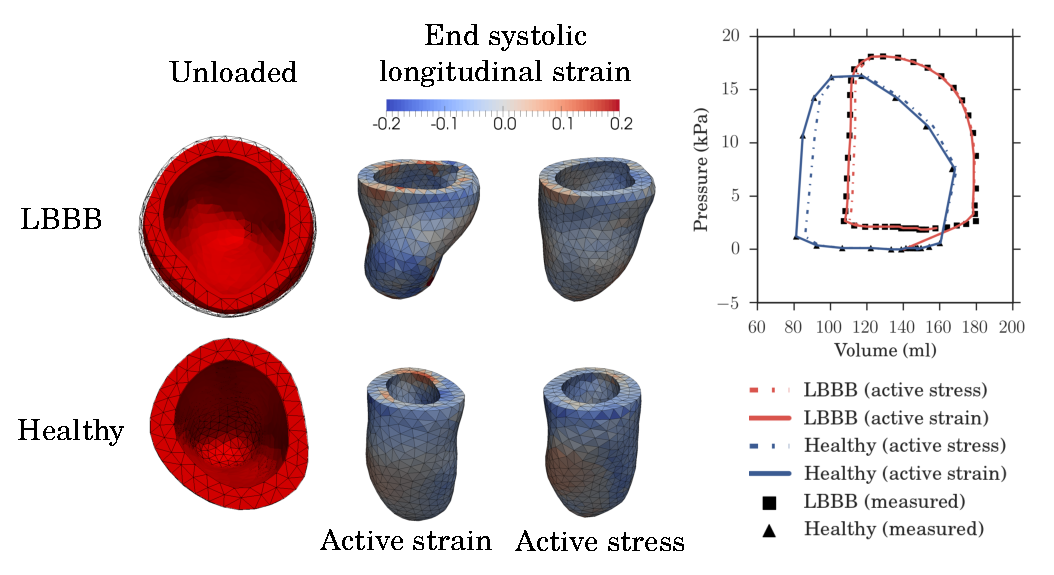
\includegraphics[width=\textwidth]{generic_result}
  \caption{Left: Snap shots of the unloaded geometry in red, and the
    corresponding image based geometry taken at beginning of atrial
    systole in black wire-frame. Middle: Snap shot of end systolic
    configurations using the active strain and active stress approach.
    Color-map shows the end-systolic longitudinal strain.
    Right: Simulated and measured pressure-volume loops for
    these hearts using the active strain and active stress approach.}  
  \label{fig:generic_result}
\end{figure}


The total analysis of the 14 patients involved optimizing 432 volume
measurements and 20 853 strain measurements. The average time for one
forward and gradient evaluation was 8.3 and 8.9 seconds respectively
when running on a cluster using four cores, with an average number of
control parameters being 985.

In order to visualize the overall match of simulated to measured data,
we show linear regression plots in
Figure~\ref{fig:data_matching}. These results are all based on the
active strain formulation. For
the strain, we separately consider the diastolic and systolic points,
as different types of data were used to  constrain the model in these
two phases, namely volume in the diastolic phase and strain in the
systolic phase. An excellent overall fit was obtained for the optimized
volume ($R^2=1.00$) and systolic strains ($R^2=0.95$). 
Diastolic strains, not used in the optimization, were less well
matched ($R^2=0.31$).



\begin{figure}[htbp]
  \centering
  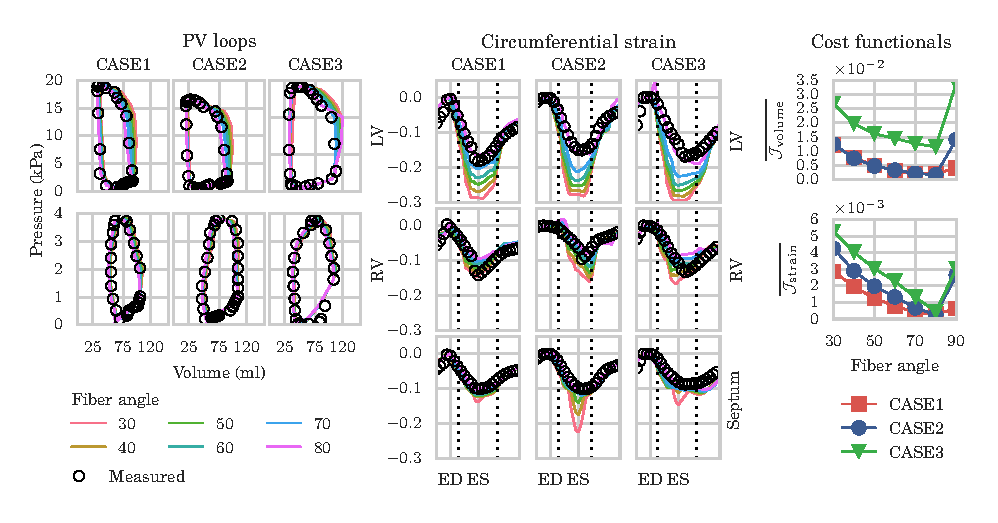
\includegraphics[width=\textwidth]{data_matching}
  \caption{Scatter plot of simulated ($y$-axis) and measured
    ($x$-axis) strain and volume using the active
    strain approach. Left: Scatter plot of simulated versus
    measured volumes and the best linear least-squares fit of these
    points, (slope = $1.00$). Right: Scatter plot of simulated versus
    measured strain for all segments and all directions, separated
    into the diastole, were only the volume was optimized and systole,
    where both the strain and volume were optimized. For diastole, the slope of
    the best linear fit was $0.31$, while the best linear fit for the
    systolic points had a slope of $0.95$.}
  \label{fig:data_matching}
\end{figure}


\subsection{Estimation of global contractility and elastance}

Global contraction time courses, $\overline{\gamma}$ and
  $\overline{T}_a$, for each patient were synchronized to the valvular
events to normalize for differing cycle lengths. The average 
and standard deviation of these normalized traces for the
LBBB vs the healthy controls are shown in left of
Figure~\ref{fig:contractility}. The healthy patients had a much higher
level of contraction through the cardiac cycle, and the peak values
were compared using one-way ANOVA, yielding a $P-$value less than
$0.001$ for both the active strain and the active stress approach. 

The values of calculated $\tilde{E}\es$ for the healthy and LBBB patients are
shown to the right in Figure~\ref{fig:contractility}. The calculated
elastances of the LBBB group were significantly lower than for the healthy
group, with the comparison between the groups using one-way ANOVA
giving a $P-$value of $0.009$ and $0.003$ for the active strain and
active stress respectively.




\begin{figure}[htbp]
  \centering
  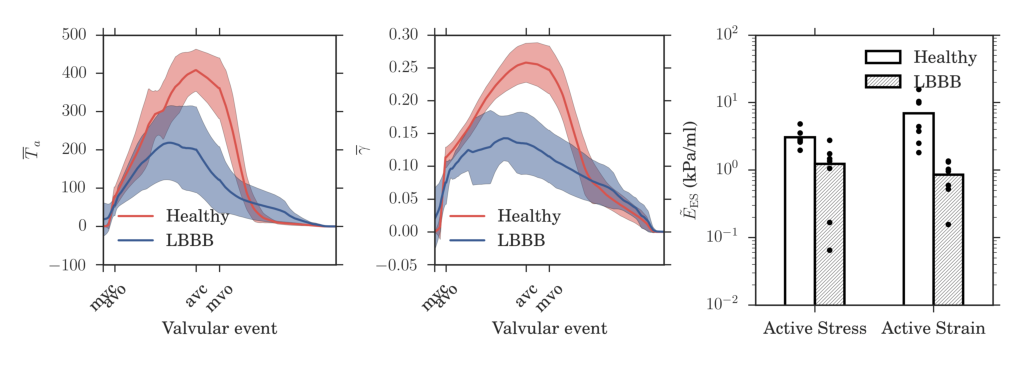
\includegraphics[width=\textwidth]{contractility}
  \caption{Extracted biomarkers related to cardiac contractility.
    Left:  Mean value of $T_a$ for the two groups
    synchronized with respect to valvular events (mvc: mitral valve
    closure, avo: aortic valve opening, avc: aortic valve closure,
    mvo: mitral valve opening). Shaded region shows $\pm$ one standard
    deviation.
    Middle:  Mean value of $\gamma$ for the two groups
    synchronized with respect to the same valvular events.
    Right: Estimated values of $\tilde{E}\es$, given by
    \eqref{eq:estimate_elastance} using the active stress and the
    active strain approach. The mean value is depicted for each
    group as a bar, and individual points are also displayed.} 
  \label{fig:contractility}
\end{figure}



\section{Discussion}
In this study we applied an adjoint-based data assimilation technique
to constrain patient data to a cardiac mechanics model.
LV pressure was used as a boundary condition,  and an unloading algorithm was used to 
find a reference geometry and a material parameter based on diastolic P-V measurements.  
Active contraction was then captured by assimilation of measured systolic LV
regional strains by the means of a
spatially varying contraction parameter.  We tested this methodology on a group of
seven healthy control patients and seven patients
diagnosed with LBBB. The results gave an excellent fit between the measured
and simulated volume and systolic strain ($R^2 \geq 1.00$ and $R^2
\geq 0.95$, respectively) for more than 21,000 observation points.
Meanwhile diastolic strains, due to the quality of the strain measurements during late
diastole, were not included in the optimization and had a
resulting poor fit.  However, allowing for spatial heterogeneity in the 
material parameters and/or optimizing more parameters from the
material model, could allow for better fit values also in this
part of the cycle and will be further investigated. Of course, questions regarding uniqueness of
such solutions in general will need to be carefully
addressed in future studies. 

Our simulations show that estimating the unloaded configuration may be important to capture the
correct material parameters, as we optimized to a consistently softer material when the unloading 
algorithm was used.  Meanwhile, this seemed to have less of an impact in systole, as the 
the overall estimated ventricular elastance was unchanged.

These calibrated models allow for estimating aspects of cardiac
contractility, such as the traditional measure of end-systolic
elastance, by perturbations of the model at the end systolic
configuration.  The healthy control group had significantly higher estimated
end-systolic elastance than the LBBB group, although limitations exist
with these calculations due to using a synthetic pressure curve with
the healthy group.  However, the values calculated by using direct
pressure readings for the LBBB group (3 - 10 mmHg) are slightly higher
but correspond very well with the range provided for a heart failure
cohort of (0.5 - 4.9 mm Hg) \cite{senzaki1996single}. Clinically, end systolic elastance is measured
based on data obtained using multiple beats
subjected to different loading conditions. This change in loading
conditions  also gives rise to changes in the active tension as a function of myocardial strain,
an effect that is not modelled directly here.  Therefore, although we can calculate a discriminating marker of
stiffness between the two cohorts, future work evaluating this method over a number of beats
with different loading conditions is needed to assess its relation to clinical end-systolic elastance.

In addition to the end-systolic elastance estimates, our simulations also were used to
compare the average value of $\gamma$ and $T_a$, which may also be
interpreted as indices of contractility, between the two groups
through the cardiac cycle. Again, the healthy controls showed a
significantly higher peak values of active strain and stress, compared
to the LBBB group and both  analysis methods showed comparable trends. 


\section{Conclusions}

Adjoint-based data assimilation is a powerful technique for
estimating high dimensional parameters in order to incorporate large
amounts of information into a model. Although limitations in our
patient data and assumptions remain, we have demonstrated how such
techniques can be applied to problems in mechanics for use in
extracting potential biomarkers related to cardiac
contractility. Future work will be used to adjust and improve such
models and work towards their validation and clinical utility.


\section*{Acknowledgments}
This study was funded by Research Council of Norway: Center for
Biomedical Computing at Simula Research Laboratory and Center for
Cardiological Innovation at Oslo University Hospital.
%, grant number 179578 and 203489.
Computations were performed on the Abel supercomputing cluster at the 
University of Oslo via a Notur project.
% project nn9249k.

% \pagebreak
\newpage
\bibliographystyle{plain}
\bibliography{chapters/paper2/bibliography}

%%% Local Variables:
%%% mode: latex
%%% TeX-master: "../../main"
%%% End:
